% !TEX program = pdflatex
% ============================================================
% Manuscript: Interferon activation and nCRT response in LARC
% Single-column submission version, TeX Live 2026, pdflatex
% Numbers follow manuscript_draft.md (audit version 2026-09-12)
% ============================================================
\documentclass[11pt,a4paper]{article}

\usepackage[T1]{fontenc}
\usepackage[utf8]{inputenc}
\usepackage{lmodern}
\usepackage{microtype}
\usepackage{graphicx}
\usepackage{xcolor}
\usepackage{geometry}
\usepackage{booktabs}
\usepackage{tabularx}
\usepackage{adjustbox}
\usepackage{enumitem}
\usepackage[labelfont=bf]{caption}
\usepackage[numbers,sort&compress]{natbib}
\usepackage{lineno}
\usepackage{amsmath}

\geometry{a4paper, top=2.5cm, bottom=2.5cm, left=2.5cm, right=2.5cm}

% hyperref last
\usepackage[colorlinks=true,linkcolor=blue,citecolor=blue,urlcolor=blue,
            bookmarks=true,unicode=true]{hyperref}

\widowpenalty=10000
\clubpenalty=10000
\setlength{\bibsep}{2pt}

\newcommand{\posg}{Positive Hedges $g$ denotes higher scores in responders.}

\begin{document}

% ---------------- Title block ----------------
\begin{center}
{\LARGE\bfseries Pretreatment interferon activation and cytotoxic immune enrichment are associated with response to neoadjuvant chemoradiotherapy in locally advanced rectal cancer: a systematic multi-cohort transcriptomic meta-analysis\par}
\vspace{1.2em}
{\large Bizhi Wei\par}
\vspace{0.4em}
{\small Puai Medical College, Shaoyang University, Shaoyang, Hunan, China\par}
\vspace{0.4em}
{\small Corresponding author: Bizhi Wei, Puai Medical College, Shaoyang University, Shaoyang, Hunan, China. Email: 15619056250wbz@gmail.com; ORCID: 0009-0008-9481-3024\par}
\vspace{0.4em}
{\small Running title: Interferon activation and nCRT response in rectal cancer\par}
\end{center}

\vspace{0.8em}
\noindent\textbf{Manuscript type:} Original Article.

% ---------------- Abstract ----------------
\section*{Abstract}
\noindent\textbf{Background.} Transcriptomic markers of response to neoadjuvant chemoradiotherapy (nCRT) in locally advanced rectal cancer (LARC) have uncertain reproducibility across cohorts. We examined whether pretreatment immune states show consistent associations with response across public datasets.

\noindent\textbf{Methods.} A systematic search and post-search audit assessed 41 neoadjuvant rectal-cancer transcriptomic datasets. Nine response-classified nCRT cohorts formed the primary analysis ($n=577$). A radiotherapy-only cohort ($n=51$ independent patients) was restricted to a regimen-scope sensitivity analysis. Within each cohort, we calculated interferon (IFN), cytotoxic-lymphocyte and natural killer (NK)-cell scores by single-sample gene-set enrichment analysis. Standardized effects were pooled as Hedges $g$ using random-effects meta-analysis with modified Hartung--Knapp inference.

\noindent\textbf{Results.} \posg{} IFN scores were higher in responders in eight of nine nCRT cohorts ($g=0.38$, 95\% CI 0.16--0.61; $P=0.0041$; $I^2=1\%$). The IFN association remained positive across three alternative signatures, three core genes (\textit{STAT1}, \textit{CXCL10}, \textit{IFNG}) and an alternative $z$-score scoring method ($g=0.28$--$0.39$, all $P<0.035$). Cytotoxic-lymphocyte scores were also higher in responders ($g=0.26$, 95\% CI 0.04--0.49; $P=0.026$); this association was reproduced with the official MCPcounter implementation ($g=0.31$, $P=0.025$), whereas the MCPcounter NK estimate remained uncertain ($g=0.21$, $P=0.072$). The continuous NK-cell estimate was less precise ($g=0.23$, 95\% CI $-0.005$ to 0.47; $P=0.054$). All three effects were negative in the radiotherapy-only cohort, and the treatment-scope sensitivity estimate (nine nCRT cohorts plus RT-only GSE56699) was attenuated ($g=0.30$, 95\% CI 0.04--0.56; $P=0.030$; $I^2=34\%$). In available-subset analyses, IFN estimates remained directionally positive after adjustment for measured clinical, stromal and genomic variables. Adding IFN to clinical T and N stage in GSE87211 improved model fit in-sample (likelihood-ratio $P=0.016$); the optimism-corrected AUC increment was 0.049 (95\% CI $-0.058$ to 0.136). IFN was not associated with disease-free survival after pathological-stage adjustment (HR$=1.05$, $P=0.80$).

\noindent\textbf{Conclusions.} Pretreatment interferon activation and cytotoxic immune enrichment were reproducibly associated with nCRT response across heterogeneous transcriptomic cohorts. Their treatment specificity, incremental value and clinical utility require prospective validation with prespecified models and thresholds.

\vspace{0.5em}
\noindent\textbf{Keywords:} rectal cancer; neoadjuvant chemoradiotherapy; interferon; tumor microenvironment; NK cells; meta-analysis; complete response; watch-and-wait

\linenumbers

% ---------------- Introduction ----------------
\section{Introduction}

Neoadjuvant chemoradiotherapy (nCRT) followed by total mesorectal excision remains an established treatment for locally advanced rectal cancer (LARC) \cite{Sauer}. Response varies substantially, from limited regression to pathological complete response. Patients who achieve a sustained clinical complete response may also enter structured organ-preservation programs \cite{GarciaAguilar}. Pretreatment markers that reliably identify response-associated biology could therefore improve trial stratification and guide biomarker development.

Many transcriptomic response signatures have been reported, yet their transportability remains uncertain. Public cohorts differ in assay platform, treatment regimen and response definition. Endpoints include sustained complete response, pathological complete response and several tumor-regression grading systems. These differences limit direct pooling of expression values and can make apparent validation dependent on one dataset or coding decision. A quantitative synthesis based on within-cohort standardized effects can separate reproducible biological signals from cohort-specific signatures.

Immune activation is a plausible cross-cohort signal because several rectal-cancer studies have linked interferon signaling or cytotoxic immune states to treatment response \cite{Akiyoshi,Chatila,Alderdice}. However, these associations have not been quantitatively synthesized using harmonized within-cohort standardized effects across systematically audited public nCRT cohorts. It also remains unclear whether any association persists across alternative gene sets or after accounting for measured clinical and tumor-composition variables.

We therefore conducted a systematic multi-cohort reanalysis of pretreatment rectal-cancer transcriptomes. Nine nCRT cohorts containing 577 response-classified tumors formed the primary analysis. A radiotherapy-only cohort was reserved for a regimen-scope sensitivity analysis. We harmonized pathway and immune-marker scores within cohorts, pooled standardized effects, and tested the main IFN finding across alternative signatures. We also examined selected clinical, stromal and genomic covariates where public data permitted.

% ---------------- Methods ----------------
\section{Materials and Methods}

\subsection{Systematic cohort identification and eligibility}

We searched GEO DataSets on 1 September 2026 using the following query:
\begin{quote}\small\texttt{%
(rectal[Title]) AND (neoadjuvant OR chemoradiotherapy OR \\
chemoradiation OR radiochemotherapy) AND ("expression profiling by array" \\
OR "expression profiling by high throughput sequencing")[Filter] \\
AND "Homo sapiens"[Organism]}\end{quote}

Eligible datasets contained human rectal tumors sampled before neoadjuvant treatment, bulk transcriptomic profiles, public sample-level response labels and obtainable probe annotations. We assessed 41 datasets and excluded 31 for documented reasons (Supplementary Methods; Figure~S0). Nine nCRT cohorts containing 577 response-classified tumors formed the primary synthesis. GSE56699 included 51 independent patients treated with preoperative radiotherapy alone \cite{Isella} and entered a regimen-scope sensitivity analysis. GSE213331 was assessed and excluded: its 18 response-labelled samples are post-treatment resected tissues (nine pCR, nine non-pCR), whereas its only pretreatment samples (nine biopsies) carry no response label, so it cannot contribute to a pretreatment response association \cite{He}. GSE216616, the largest identified dataset ($n=298$ \cite{Akiyoshi}), was ineligible because sample-level response labels were not deposited. TCGA-READ provided non-nCRT prognostic context only. It comprised 164 treatment-naive primary tumors after excluding one neoadjuvantly treated sample.

\subsection{Response definitions}

Response endpoints followed the source publications and deposited metadata. GSE209746 used sustained two-year complete response (CR) versus incomplete response (iCR) from the source study's Table~S1A \cite{Chatila}. Of 94 reported patients, one lacked GEO RNA data. GSE87211 used pathological complete response (pCR), defined as ypT0N0 \cite{Hu}. One of 203 tumors was excluded because both ypT and ypN were missing.

GSE35452 \cite{Watanabe}, GSE150082 \cite{Sendoya}, GSE45404 \cite{Agostini} and GSE53781 \cite{Palma} used tumor-regression-grade dichotomies. GSE119409 used deposited sensitivity labels \cite{Ji}, and GSE133057 used AJCC/CAP regression scores 0--1 versus 2--3 \cite{Ferrandon}. GSE94104 used pretreatment biopsies and its reported ascending scale, with TRG3 classified as favorable and TRG1--2 as poor response \cite{Alderdice}. For GSE56699, we restricted the official SDRF to pretreatment biopsies and classified Mandard TRG1--2 versus TRG3--5. One patient without a Mandard grade was excluded. GSE56699 did not enter the primary nCRT analysis. Table~S1 records each source definition, metadata field, final coding and manual verification.

\subsection{Expression preprocessing and harmonized scoring}

RNA-sequencing counts from GSE209746 and TCGA-READ were mapped to gene symbols and transformed as $\log_2(\mathrm{CPM}+1)$. GSE209746 was also modeled with DESeq2 using Wald tests, Benjamini--Hochberg correction and a total-count threshold of 10 \cite{Love}. Microarray matrices were used as submitted after scale checks. Platform-specific annotations mapped probes to gene symbols. The highest-variance probe represented genes mapped by multiple probes.

We did not merge expression matrices across cohorts. Scores and effects were calculated within each cohort, then combined at the effect-size level (Table~S2). GSE56699 required an additional independence correction because 58 pretreatment arrays represented 52 patients. Repeated biopsies were averaged within patient on the expression scale before scoring. Excluding one patient without a Mandard grade yielded 51 independent patients. Reversing the operation order, by scoring each array before patient-level averaging, produced nearly identical scores (Spearman $\rho=0.994$--$0.999$).

Per-sample scores were calculated by single-sample gene-set enrichment analysis (ssGSEA) in GSVA \cite{Hanzelmann}. The IFN score was the mean of HALLMARK\_INTERFERON\_ALPHA\_RESPONSE and HALLMARK\_INTERFERON\_GAMMA\_RESPONSE ssGSEA scores \cite{Liberzon}. Immune and stromal scores used published MCP-counter marker sets \cite{Becht}. This implementation is a marker-set score, not the MCPcounter package's cell-abundance estimate. The scores correlated with published Bindea scores in the discovery cohort ($r=0.87$--$0.96$) \cite{Bindea}. Hallmark competitive testing used camera \cite{Wu} in limma \cite{Ritchie}.

We tested three alternative IFN definitions: the Ayers six-gene IFN-$\gamma$ signature \cite{Ayers}, Reactome Interferon Alpha/Beta Signaling and Reactome Interferon Gamma Signaling. The Ayers signature comprised \textit{IFNG}, \textit{STAT1}, \textit{IDO1}, \textit{CXCL9}, \textit{CXCL10} and \textit{HLA-DRA}. We also examined single-gene scores for \textit{CXCL9}, \textit{CXCL10}, \textit{IDO1}, \textit{STAT1} and \textit{IFNG}. Two additional implementation checks addressed scoring method and immune-cell scoring approach. First, we replaced ssGSEA with a cohort-internal gene-wise $z$-score mean of the same Hallmark IFN genes (mean-$z$ score). Second, we recomputed NK-cell and cytotoxic-lymphocyte scores with the official MCPcounter abundance-estimation procedure, rather than the ssGSEA marker-set implementation, using its published gene signatures.

For the clinical association model, apparent incremental AUC of the IFN score beyond clinical T/N stage was corrected for optimism by the Efron--Gong bootstrap (2000 resamples), comparing the full model against the clinical model within each resample. Survival associations were additionally examined in a sequential adjustment framework (ypT+ypN, then +IFN, then +age and sex) reporting the IFN hazard ratio, concordance index and model-comparison likelihood-ratio tests at each step.

\subsection{Immune subgroups}

Discovery-cohort immune groups were reconstructed from the original study \cite{Chatila}. All microsatellite-instability (MSI) tumors formed IG4. Microsatellite-stable (MSS) tumors were clustered by $k$-means using $z$-scored ssGSEA values for 22 Bindea immune populations. We used $k=3$ and \texttt{nstart}=50, then ordered clusters from IG1 (cold) to IG3 (hot). Cluster stability was assessed across 50 random seeds.

\subsection{Effect sizes, meta-analysis and diagnostics}

For each cohort and feature, we calculated Hedges $g$ with a small-sample correction. Effects compared responders with poor responders, so positive values indicate higher scores in responders. The IFN score was the primary feature. The cytotoxic-lymphocyte score provided supporting evidence, and the NK-cell score was treated as sensitivity evidence.

Random-effects models estimated $\tau^2$ by restricted maximum likelihood (REML). Confidence intervals used modified Hartung--Knapp inference with the variance multiplier constrained to at least one. We report $\tau^2$, Cochran's $Q$, $Q$ degrees of freedom and $I^2$ for each pooled estimate. DerSimonian--Laird estimates provided a model sensitivity analysis. Prediction intervals used a $t$ distribution with $k-2$ degrees of freedom \cite{IntHout}.

Diagnostics comprised leave-one-cohort-out analyses, Baujat plots and Egger regression. Baujat plots compared each cohort's heterogeneity contribution with its influence on the pooled estimate. Egger tests were considered low-powered because the primary analysis contained nine cohorts. A coverage sensitivity analysis excluded GSE133057 and GSE53781, which had less than 80\% probe annotation. A regimen-scope analysis added the radiotherapy-only cohort. This analysis evaluated transport across treatment contexts and did not replace the nCRT primary model.

We further tested response-definition sensitivity within the nine nCRT cohorts by classifying endpoints as complete-response endpoints (sustained CR in GSE209746; pCR $=$ ypT0N0 in GSE87211) versus broader response-classification endpoints (TRG-based or sensitivity/resistance coding in the remaining seven cohorts). Subgroup pooling used the same REML--modified Hartung--Knapp model. Prediction intervals were omitted for the complete-response subgroup because only two cohorts were available ($k-2=0$ degrees of freedom). The complete-response subgroup and the subgroup-difference test were considered exploratory and interpreted primarily for direction and magnitude. Within GSE87211, regimen sensitivity compared fluoropyrimidine chemoradiotherapy (5-FU $+$ RT) with an oxaliplatin-containing stratum (5-FU $+$ oxaliplatin $\pm$ cetuximab $+$ RT); the small cetuximab arm was merged with the oxaliplatin-containing stratum. Stratified Hedges $g$ and a score $\times$ regimen interaction term in a linear model of the $z$-scored immune score ($z(\mathrm{score}) \sim \mathrm{response} * \mathrm{regimen}$) assessed whether the score--response association differed by regimen.

We also compared each cohort's top score tertile with its lower two tertiles. Log odds ratios were pooled with the same random-effects framework. The tertile threshold was chosen in advance and was not optimized against response. We therefore treated this analysis as a sensitivity analysis rather than independent validation.

\subsection{Confounder analyses}

MSI status was available for the discovery cohort, including five MSI tumors. We used MSI-adjusted DESeq2 models, an MSS-only sensitivity analysis ($n=85$) and Fisher exact tests. Selected linear and logistic models included fibroblast and endothelial marker-set scores. In the discovery cohort's whole-exome-sequencing subset, we examined tumor purity, tumor mutational burden, copy-number-altered fraction and whole-genome doubling. GSE87211 mutation data supported a KRAS-adjusted IFN--pCR model. These cohort-specific analyses addressed measured covariates but could not exclude residual confounding.

\subsection{Predictive performance and incremental association}

Receiver-operating-characteristic curves and areas under the curve (AUCs) were calculated with pROC \cite{Robin}. In GSE87211, 197 tumors had complete clinical T and N stage. Logistic models compared clinical stage alone with clinical stage plus the IFN score. We used a likelihood-ratio test for nested models and a DeLong test for apparent AUCs. Interpretation followed the bootstrap-corrected incremental association described above rather than validated clinical utility.

\subsection{Survival analysis}

GSE87211 disease-free survival (DFS) included 175 patients and 34 events. Overall survival (OS) included 175 patients and 21 events. Cox models were fitted univariably, after adjustment for ordinal ypT and ypN, and after additional age and sex adjustment. We tested nonlinearity with a three-degree-of-freedom natural spline and performed pCR-stratified analyses. Median follow-up was calculated by the reverse Kaplan--Meier method. TCGA-READ OS and progression-free interval used curated endpoints \cite{Liu} and were modeled with and without AJCC-stage adjustment.

\subsection{Statistics and software}

Analyses used R 4.6.1 with DESeq2 1.52.0, limma 3.68.4, GSVA 2.6.3, pROC 1.19.1 and survival 3.8-6. REML estimation of $\tau^2$ and modified Hartung--Knapp intervals were implemented in project code (pool\_random\_effects in meta\_utils.R, following the variance-component and multiplier formulations of IntHout et al.~\cite{IntHout}); no meta-analysis package was used. The MCPcounter sensitivity analysis used the official MCPcounter package (ebecht/MCPcounter, GitHub master) with its published gene signatures. Tests were two-sided with $\alpha=0.05$. Genome-wide analyses used Benjamini--Hochberg false-discovery-rate control. Complete package versions are recorded in the analysis log. Analysis scripts, label provenance and output mappings are described in the Data availability statement.

% ---------------- Results ----------------
\section{Results}

\subsection{Systematic assembly of the primary and sensitivity cohorts}

The systematic search and post-search audit assessed 41 datasets and excluded 31 for documented reasons. Exclusions included absent sample-level response labels for GSE216616 ($n=298$) and GSE109057 ($n=91$). The primary synthesis contained nine nCRT cohorts and 577 response-classified pretreatment tumors. GSE56699 contributed 51 independent radiotherapy-only patients to a regimen-scope sensitivity analysis. The combined dataset comprised 628 patients across 10 cohorts (Table~\ref{tab:cohorts}; Figure~S0).

\subsection{Discovery reproduction and the 15-gene resistance signature}

DESeq2 reproduced the direction of all 15 genes in the discovery resistance signature. In the MSS-only analysis, 14 genes met $|\log_2\mathrm{FC}|>1$ and FDR$<0.05$. This set included \textit{CPS1}, which did not meet both thresholds in the full cohort. Across five cohorts, 11 of 14 evaluable genes retained the expected direction in REML-mKH meta-analysis. No gene survived Benjamini--Hochberg correction. \textit{INHBB} ($g=-0.52$, $P=0.024$, FDR$=0.324$) and \textit{KLK6} ($g=-0.32$, $P=0.046$, FDR$=0.324$) had the smallest nominal $P$ values (Figure~S5; Table~S3). MSI-adjusted discovery models retained \textit{IGF2} (FDR$=4.3\times10^{-7}$) and \textit{L1CAM} (FDR$=7.8\times10^{-4}$).

\subsection{Interferon signaling was consistent across the initial cohorts}

Competitive Hallmark testing showed higher interferon-$\alpha$ and interferon-$\gamma$ pathway activity in responders across the four initial cohorts. IFN-$\alpha$ $P$ values ranged from $7.2\times10^{-3}$ to $9.0\times10^{-18}$. IL6-JAK-STAT3 and inflammatory-response pathways generally followed the same direction. Oxidative-phosphorylation and glycolysis pathways were generally lower in responders, whereas hypoxia, proliferation and epithelial-mesenchymal-transition pathways were inconsistent (Figure~S1).

\subsection{Primary nine-cohort nCRT meta-analysis}

The pretreatment IFN score was the designated primary feature. Scores were higher in responders in eight of nine nCRT cohorts. The pooled estimate was $g=0.38$ (95\% CI 0.16--0.61; $P=0.0041$; $I^2=1\%$; $\tau^2=0$; $Q=8.12$, df$=8$, $P=0.42$; Figure~\ref{fig:main}A). Because estimated between-cohort variance was zero, the prediction and confidence intervals were similar. At three decimals, the 95\% prediction interval was 0.156--0.611, compared with a confidence interval of 0.161--0.606.

Cytotoxic-lymphocyte scores were higher in responders in seven of nine cohorts ($g=0.26$, 95\% CI 0.04--0.49; $P=0.026$; $I^2=0\%$; $\tau^2=0.003$). The 95\% prediction interval was 0.003--0.52. The continuous NK-cell estimate was similar but less precise ($g=0.23$, 95\% CI $-0.005$ to 0.47; $P=0.054$; $I^2=0\%$; $\tau^2=0.012$). Its prediction interval ranged from $-0.12$ to 0.59 (Figure~\ref{fig:main}B).

Leave-one-cohort-out IFN estimates ranged from 0.34 to 0.43 and remained nominally significant ($P=0.0036$--$0.020$). NK and cytotoxic estimates lost nominal significance after some cohort omissions (Figure~S2; Table~S4). In Baujat analyses, GSE150082 contributed most to IFN heterogeneity. GSE87211 had the largest influence on the NK and cytotoxic estimates, consistent with its greater weight. No cohort combined a large heterogeneity contribution with high influence on a pooled estimate (Figure~S2). Egger tests gave $P=0.58$ for IFN, $P=0.24$ for NK and $P=0.050$ for cytotoxic scores. These tests were based on only nine cohorts.

The high-annotation-coverage analysis retained seven nCRT cohorts. Estimates were $g=0.45$ for IFN (95\% CI 0.20--0.70; $P=0.0046$), $g=0.32$ for cytotoxic scores (95\% CI 0.07--0.57; $P=0.020$) and $g=0.26$ for NK scores (95\% CI $-0.03$ to 0.54; $P=0.072$).

By contrast, all three effects were negative in radiotherapy-only GSE56699 (IFN $g=-0.32$; NK $g=-0.19$; cytotoxic $g=-0.16$).

The treatment-scope sensitivity analysis (nine nCRT cohorts plus RT-only GSE56699) reduced the pooled estimates and increased IFN heterogeneity. The IFN estimate was $g=0.30$ (95\% CI 0.04--0.56; $P=0.030$; $I^2=34\%$), with a prediction interval of $-0.24$ to 0.84. The corresponding $P$ values were 0.106 for NK and 0.058 for cytotoxic scores (Table~\ref{tab:meta}).

\subsection{Response-definition and regimen sensitivity}

In the complete-response subgroup (GSE209746 and GSE87211; $k=2$, $n=295$), both cohort estimates were positive and the pooled point estimate was $g=0.40$; the exploratory confidence interval was very wide because modified Hartung--Knapp inference with one residual degree of freedom is unstable at $k=2$, and no prediction interval was computed. In the broader response-classification subgroup ($k=7$, $n=282$), the pooled IFN estimate was $g=0.37$ (95\% CI 0.02--0.72; $P=0.043$; $I^2=21\%$), with six of seven cohort estimates positive. Cochran $Q$ decomposition gave no evidence of effect modification by response-definition class for IFN ($P_{\mathrm{between}}=0.89$), NK ($P_{\mathrm{between}}=0.19$) or cytotoxic scores ($P_{\mathrm{between}}=0.26$). Effects were positive under both endpoint classes, with no evidence of effect modification by response-definition class; the subgroup comparison was underpowered, particularly because the strict complete-response subgroup contained only two cohorts.

Within GSE87211, the 202 response-evaluable tumors comprised 111 treated with fluoropyrimidine CRT and 91 in the oxaliplatin-containing stratum, which included the small cetuximab arm. Both strata showed positive IFN effects (Hedges $g=0.47$ and $0.54$). Score $\times$ regimen interaction terms were not significant for IFN ($P=0.70$), NK ($P=0.79$) or cytotoxic scores ($P=0.19$). The pretreatment score--response association was therefore not restricted to either regimen stratum in this cohort.

\subsection{Robustness across IFN definitions, scoring methods and immune-scoring implementations}

All three alternative IFN signatures produced positive estimates across the nine nCRT cohorts. The Ayers six-gene IFN-$\gamma$ signature gave $g=0.29$ (95\% CI 0.03--0.55; $P=0.034$). Reactome IFN-$\alpha/\beta$ and IFN-$\gamma$ signaling gave $g=0.35$ (95\% CI 0.12--0.58; $P=0.008$) and $g=0.33$ (95\% CI 0.07--0.60; $P=0.019$), respectively. Within cohorts, alternative scores correlated with the primary IFN score at Spearman $\rho=0.58$--$0.92$.

Single-gene analyses were positive for \textit{STAT1} ($g=0.39$, 95\% CI 0.15--0.63; $P=0.006$), \textit{CXCL10} ($g=0.32$, 95\% CI 0.08--0.56; $P=0.017$) and \textit{IFNG} ($g=0.28$, 95\% CI 0.06--0.50; $P=0.019$). \textit{CXCL9} and \textit{IDO1} were positive but did not reach nominal significance (Figure~S7; Table~S8).

Replacing ssGSEA with the cohort-internal mean-$z$ scoring method gave $g=0.38$ (95\% CI 0.14--0.61; $P=0.0066$; 8/9 direction-consistent), with a median within-cohort Spearman correlation of 0.94 against the ssGSEA score. Recomputing the supporting cell scores with the official MCPcounter package likewise reproduced the synthesis (cytotoxic $g=0.31$, 95\% CI 0.05--0.57, $P=0.025$; NK $g=0.21$, $P=0.072$; within-cohort Spearman $\rho=0.93$--$0.95$ versus the ssGSEA implementation). The IFN association was robust to gene-set definition and scoring method. The cytotoxic-immune association was also reproduced using official MCPcounter abundance estimates.

\subsection{Within-cohort top-tertile sensitivity analysis}

Reconstructed discovery-cohort immune subgroups reproduced the published CR gradient: IG1 26\%, IG2 22\%, IG3 67\% and IG4 (MSI) 60\%. The combined IG3/4 response rate was 64\% versus 24\% for IG1/2 (Fisher $P=0.012$; MSS-only 67\% vs 24\%, $P=0.043$; stable across 50 clustering seeds; Figure~\ref{fig:main}C). In a separate top-tertile analysis, the NK-high group had greater odds of response (OR$=1.98$, 95\% CI 1.13--3.44; $P=0.022$; $I^2=24\%$). Its prediction interval was wide and crossed one (0.70--5.54). IFN (OR$=1.66$, 95\% CI 0.98--2.80, $P=0.056$) and cytotoxic-high status (OR$=1.57$, 95\% CI 0.92--2.71, $P=0.090$) did not reach nominal significance (Figure~S3; Table~S5).

\subsection{Available-subset covariate analyses}

The IFN estimate was positive in the MSS-only analysis ($g=0.35$), compared with $g=0.28$ in the full discovery cohort. MSI-adjusted analyses gave the same direction. Stromal marker-set scores were not associated with response in the tested models (all $P>0.09$). The IFN term remained associated after stromal adjustment in GSE87211 ($P=0.005$) and GSE150082 ($P=0.006$).

The discovery cohort's whole-exome-sequencing subset contained 57 patients. Tumor mutational burden, purity, copy-number-altered fraction and whole-genome doubling were not individually associated with response (all $P\geq0.15$). The IFN coefficient remained positive but decreased from 0.35 to 0.26 after covariate adjustment. In GSE87211, the observed pCR rate was 12\% in KRAS-mutant tumors and 20\% in wild-type tumors (Fisher $P=0.17$). The IFN term remained associated after KRAS adjustment ($P=0.0088$). These available-subset analyses did not address unmeasured confounding.

\subsection{Incremental clinical association}

IFN-score AUCs ranged from 0.556 to 0.764 across the original four cohorts. A fixed-coefficient IFN+\textit{IGF2}+\textit{L1CAM} score did not transfer consistently (Figure~S4). In GSE87211, the apparent AUC was 0.600 for clinical T and N stage. It increased to 0.655 after adding IFN (delta 0.055). The nested-model likelihood-ratio $P$ value was 0.016, and the DeLong $P$ value was 0.21. In a 2000-resample optimism bootstrap, the corrected delta AUC was 0.049 (95\% CI $-0.058$ to 0.136): the increment was stable in magnitude but its confidence interval included the null, consistent with an association measurable at cohort scale rather than a validated single-patient discriminator.

\subsection{Response-linked outcome patterns}

Median follow-up in GSE87211 was 71.2 months. Patients with pCR had no observed recurrences, compared with 34 events among 143 non-pCR patients (log-rank $P=0.003$; Figure~\ref{fig:main}D). A Cox model could not be estimated within the pCR subgroup because it contained no events. After ypT and ypN adjustment, the pretreatment IFN score was not associated with DFS (HR$=1.05$, 95\% CI 0.72--1.54; $P=0.80$) or OS (HR$=0.94$; $P=0.80$). We found no evidence of nonlinearity (spline $P=0.44$) or an association within non-pCR tumors (HR$=1.01$).

In TCGA-READ, the IFN score was not associated with OS (HR$=0.92$; $P=0.70$), including after stage adjustment ($P=0.76$). The NK marker-set score was associated with longer progression-free interval (HR$=0.70$, 95\% CI 0.51--0.97; $P=0.031$). In sequential adjustment within GSE87211, adding IFN to ypT+ypN changed the concordance index from 0.675 to 0.680 (IFN HR$=1.07$, $P=0.74$), and further adjustment for age and sex left the IFN term non-significant (HR$=1.05$, $P=0.81$; c-index 0.713); the concordance gain arose mainly from age, not IFN (Table~S7).

% ---------------- Discussion ----------------
\section{Discussion}

\subsection{Principal findings}

Across nine public nCRT cohorts, pretreatment IFN activation showed the most consistent association with response. Cytotoxic-lymphocyte scores provided concordant supporting evidence. Positive results across three alternative IFN signatures, three core genes, two scoring methods (ssGSEA and mean-$z$), and reproduction of the cytotoxic-immune association with official MCPcounter abundance estimates reduced dependence on any single analytical choice. The association was also positive under both complete-response and broader response-classification endpoint classes, and within GSE87211 it was present in both fluoropyrimidine-based and oxaliplatin-containing CRT strata. These analyses support an interferon-active response-associated state within the nCRT setting.

The evidence was weaker for NK-cell scores. The continuous estimate narrowly included the null under modified Hartung--Knapp inference. A top-tertile analysis was nominally positive, but its prediction interval included no association in a future cohort. We therefore regard NK-cell enrichment as sensitivity evidence rather than a primary finding.

Treatment context marked an important boundary. IFN, NK and cytotoxic effects were negative in the radiotherapy-only cohort, and the pooled IFN estimate weakened when this cohort was combined with the nCRT set. This contrast does not establish a treatment interaction because cohort, endpoint and platform also differed. It does show that the nCRT association should not be assumed to transport unchanged to radiotherapy alone.

The covariate, clinical-stage and survival analyses further constrain interpretation. IFN estimates remained positive in available adjusted subsets, but these subsets were small and cohort-specific. Bootstrap optimism correction yielded a similar point estimate for the incremental AUC, but its confidence interval included zero; the clinical-stage analysis therefore does not constitute validated predictive performance. IFN was not associated with adjusted survival. The present evidence therefore supports a reproducible response association, not causal mediation, prognostic independence or clinical utility.

\subsection{Convergent independent evidence}

The findings align with several independent observations. A 298-patient JFCR RNA-sequencing study reported an association between cytotoxic-lymphocyte scores and nCRT response \cite{Akiyoshi}. That cohort was excluded here because sample-level response labels were not deposited. Alderdice and colleagues identified a post-treatment NK-like signature associated with regression grade and supported it by CD56 immunohistochemistry \cite{Alderdice}. Our pretreatment NK estimate in their GSE94104 cohort had the same direction, although the pooled continuous NK result remained uncertain. An independent six-dataset machine-learning study recently derived a 186-gene predictive signature for nCRT response \cite{Corro}, reinforcing that public-cohort synthesis is productive; it differs from the present work in selecting a single multi-gene classifier rather than testing the reproducibility of a biologically defined immune state across systematically audited cohorts. Recent stroma-immune interaction analyses likewise implicate the immune microenvironment in nCRT response \cite{Wang}.

An early-phase galunisertib plus chemoradiation study also associated the immune-rich CMS1 subtype with complete response \cite{Rajamanickam}. Complete responses to PD-1 blockade in mismatch-repair-deficient LARC provide further evidence that immune context can shape rectal-cancer treatment response \cite{Cercek}. These studies differ in treatment, timing and endpoint. They support biological plausibility but do not validate the present scores.

\subsection{Why single-gene signatures fail to travel}

The discovery 15-gene resistance panel transported less consistently than the pathway-level features. Eleven of 14 evaluable genes retained the expected direction, but none survived multiple-testing correction. \textit{INHBB} and \textit{KLK6} had nominal associations and remain exploratory. Pathway and cell-marker scores aggregate information across genes, which may reduce sensitivity to platform coverage and single-transcript noise. Endpoint heterogeneity remains an alternative explanation and cannot be separated from platform effects in these data.

\subsection{Clinical implications}

IFN and cytotoxic-immune scores warrant prospective evaluation as stratification features. The reconstructed discovery immune groups and the pooled top-tertile analyses provide hypotheses for that work. They do not define a deployable classifier. AUCs were moderate, the DeLong comparison was not significant, and bootstrap optimism correction left the incremental AUC confidence interval including zero. Several prediction intervals also included the null.

A prospective study should lock the assay, score calculation and threshold before outcome analysis. It should compare molecular scores with standard clinical and imaging variables, then assess calibration and clinical utility. Separate validation would be needed for organ-preservation decisions or immunotherapy combinations.

\subsection{Implications for public-data reanalysis}

The study also identified recurrent data-provenance problems. GSE39582 has been described as containing 200 nCRT-treated LARC tumors \cite{Xue}, but we could not verify that annotation in its GEO record. The dataset originated from a colon-cancer classification study \cite{Marisa}. We therefore treated the claimed rectal-cancer subset as unavailable rather than as negative evidence.

Two large LARC series, GSE216616 and GSE109057, lacked deposited sample-level response labels. Label release would enable stronger validation. GSE216616 would be especially valuable as an independent cohort with a locked score and effect direction, rather than as another stratum added after model development. The same applies to the S:CORT Grampian and ARISTOTLE control-arm biopsies: their raw expression files are publicly exported by the consortium and have been processed here under the frozen score definition, but the per-sample pathological response labels are not part of the public export. The IFN signature was locked and timestamped (definition, direction convention and success criteria recorded with input-file hashes) before any response-label access, so that whichever labels become available first --- JFCR (GSE216616) or S:CORT Grampian/ARISTOTLE --- will serve as an out-of-sample test rather than a development set.

Free-text response fields also differed from curated source tables in several cohorts. Relevant discrepancies included 94-to-93 sample accounting, a patient with complete response followed by relapse, and the ascending GSE94104 regression scale. These examples support explicit label-provenance tables in public-data meta-analysis. Within-cohort rank-based scoring then permits cross-platform synthesis without direct batch correction of expression matrices.

\subsection{Limitations}

This study reanalyzed retrospective public data with heterogeneous endpoints, regimens and incomplete treatment details. GSE87211 alone included fluoropyrimidine-radiotherapy, oxaliplatin-containing chemoradiotherapy and a small cetuximab subgroup. GSE133057 and GSE53781 had incomplete probe annotation. Residual clinical and technical heterogeneity therefore remains despite within-cohort scoring.

The single non-nCRT cohort cannot isolate treatment interaction from cohort effects. GSE56699 involved preoperative radiotherapy alone and showed inverse score--response directions. It also required patient-level aggregation of repeated biopsies, although an alternative operation order produced almost identical scores.

Covariate availability was limited. MSI status was available only in the discovery cohort, and its MSS immune-hot subgroup contained six patients. Immune scores summarized MCP-counter marker sets by ssGSEA and were not formal cell-abundance estimates. The CD8 marker set contained one gene. Egger tests had low power, and the cytotoxic result was borderline for asymmetry. TCGA-READ provided treatment-naive prognostic context rather than nCRT validation. Protein-level and prospective validation remain necessary.

\subsection{Conclusions}

Across nine systematically selected nCRT cohorts, pretreatment interferon activation was reproducibly associated with response. Cytotoxic-lymphocyte enrichment provided supporting evidence, while the continuous NK-cell estimate remained uncertain. The association persisted across alternative IFN definitions but weakened outside the nCRT treatment context. These data justify prospective validation of a locked IFN score alongside established clinical and imaging features. They do not establish causal mediation or clinical utility.

% ---------------- Statements ----------------
\section*{Statements}

\noindent\textbf{Data availability.} All source cohorts are public through GEO: GSE209746, GSE35452, GSE87211, GSE150082, GSE45404, GSE119409, GSE133057, GSE53781, GSE94104 and GSE56699. The GSE56699 processed matrix, SDRF and ADF came from the official ArrayExpress/BioStudies record E-GEOD-56699. TCGA-READ was obtained through UCSC Xena. Analysis code, cohort-level feature tables, label provenance, derived-table mappings and manuscript source are available at \url{https://github.com/Bizhi-Wei/larc-ncrt-ifn-meta} (release tag \texttt{v1.0.1}). Large public raw matrices and serialized objects are not redistributed; accession-level download instructions are given in the repository README. A Zenodo archive DOI for this exact GitHub release will be linked in the final proof after repository archival is enabled.

\vspace{0.4em}
\noindent\textbf{Ethics.} Not required because this study re-analyzed de-identified public data.

\vspace{0.4em}
\noindent\textbf{Funding.} None.

\vspace{0.4em}
\noindent\textbf{Author contributions.} B.W.\ conceived the study, performed all analyses, and wrote the manuscript.

\vspace{0.4em}
\noindent\textbf{Conflicts of interest.} The author declares none.

% ---------------- Tables ----------------
\clearpage
\begin{table}[htbp]
\centering
\caption{Included datasets (primary nCRT analysis $n=577$; regimen-scope sensitivity $n=628$).}
\label{tab:cohorts}
\footnotesize
\adjustbox{max width=\textwidth, center}{%
\begin{tabular}{@{}l l l c p{6.8cm} c@{}}
\toprule
Cohort & Reference & Platform & $n$ & Response definition & Responders \\
\midrule
GSE209746 (discovery) & Chatila 2022 \cite{Chatila} & RNA-seq & 93 & Sustained 2-yr CR vs iCR & 26 (28\%) \\
GSE35452 & Watanabe 2014 \cite{Watanabe} & Affymetrix GPL570 & 46 & JSCCR regression grade & 24 (52\%) \\
GSE87211 & Hu, Gaedcke 2018 \cite{Hu} & Agilent GPL13497 & 202 & pCR = ypT0N0; 1 tumor with ypT/ypN both missing excluded & 35 (17\%) \\
GSE150082 & Sendoya 2020 \cite{Sendoya} & Agilent GPL13497 (2-color) & 39 & TRG Good/Poor & 16 (41\%) \\
GSE45404 & Agostini 2015 \cite{Agostini} & Affymetrix GPL570 & 42 & Mandard TRG & 19 (45\%) \\
GSE119409 & Ji 2020 \cite{Ji} & Affymetrix GPL570 & 56 & Sensitive vs resistant & 15 (27\%) \\
GSE133057 & Ferrandon 2020 \cite{Ferrandon} & Illumina GPL6102 & 33 & AJCC/CAP 0--1 vs 2--3 & 13 (39\%) \\
GSE53781 & Palma 2014 \cite{Palma} & CodeLink GPL18134 & 26 & TRG1-2 vs 3-5 & 10 (38\%) \\
GSE94104 & Alderdice 2017 \cite{Alderdice} & Illumina HT-12 (FFPE) & 40 & TRG3 vs TRG1-2 (ascending scale) & 11 (28\%) \\
GSE56699 (sensitivity) & Isella 2015 \cite{Isella} & Illumina WG-DASL v4 (FFPE) & 51 & Preoperative radiotherapy; Mandard TRG1-2 vs 3-5 & 23 (45\%) \\
\bottomrule
\end{tabular}}
\end{table}

\begin{table}[htbp]
\centering
\caption{Primary nine-cohort nCRT random-effects meta-analysis (REML-mKH; responders vs poor responders). Positive Hedges $g$ indicates higher scores in responders (uniform convention used throughout).}
\label{tab:meta}
\small
\adjustbox{max width=\textwidth}{%
\begin{tabular}{@{}l l c c c l c@{}}
\toprule
Feature & Pooled $g$ (95\% CI) & $P$ & $I^2$ & $\tau^2$ & 95\% PI & Consistent \\
\midrule
IFN score (primary) & 0.38 (0.16--0.61) & 0.0041 & 1\% & 0 & 0.16 to 0.61 & 8/9 \\
Cytotoxic lymphocytes & 0.26 (0.04--0.49) & 0.026 & 0\% & 0.003 & 0.003 to 0.52 & 7/9 \\
NK cells & 0.23 ($-0.005$ to 0.47) & 0.054 & 0\% & 0.012 & $-0.12$ to 0.59 & 7/9 \\
\bottomrule
\end{tabular}}
\end{table}

% Table 2 footnotes and pooled sensitivity estimates (kept out of the float
% because the combined block exceeds one page height).
\small
\noindent\begin{minipage}{\textwidth}
For IFN, the confidence and prediction intervals coincide at two decimals because $\tau^2\approx0$. At three decimals, the CI is 0.161--0.606 and the PI is 0.156--0.611. Cochran's $Q$ with df$=8$: IFN 8.12 ($P=0.42$), cytotoxic 6.22 ($P=0.62$), NK 7.79 ($P=0.45$).

\textbf{Coverage sensitivity (7 nCRT cohorts):} IFN $g=0.45$ (0.20--0.70), $P=0.0046$; cytotoxic $g=0.32$ (0.07--0.57), $P=0.020$; NK $g=0.26$ ($-0.03$ to 0.54), $P=0.072$.


\textbf{Treatment-scope sensitivity (9 nCRT + RT-only, 10 datasets):} IFN $g=0.30$ (0.04--0.56), $P=0.030$; cytotoxic $g=0.21$ ($-0.01$ to 0.43), $P=0.058$; NK $g=0.18$ ($-0.05$ to 0.42), $P=0.106$.


\textbf{Top-tertile sensitivity (9 nCRT cohorts):} NK OR$=1.98$ (1.13--3.44), $P=0.022$, PI 0.70--5.54; IFN OR$=1.66$ (0.98--2.80), $P=0.056$; cytotoxic OR$=1.57$ (0.92--2.71), $P=0.090$.

\textbf{Alternative IFN signatures (9 nCRT cohorts):} Ayers IFN-$\gamma$ six-gene $g=0.29$ (0.03--0.55), $P=0.034$; Reactome IFN-$\alpha/\beta$ $g=0.35$ (0.12--0.58), $P=0.008$; Reactome IFN-$\gamma$ $g=0.33$ (0.07--0.60), $P=0.019$.
\end{minipage}

% ---------------- Figure ----------------
\begin{figure}[htbp]
\centering
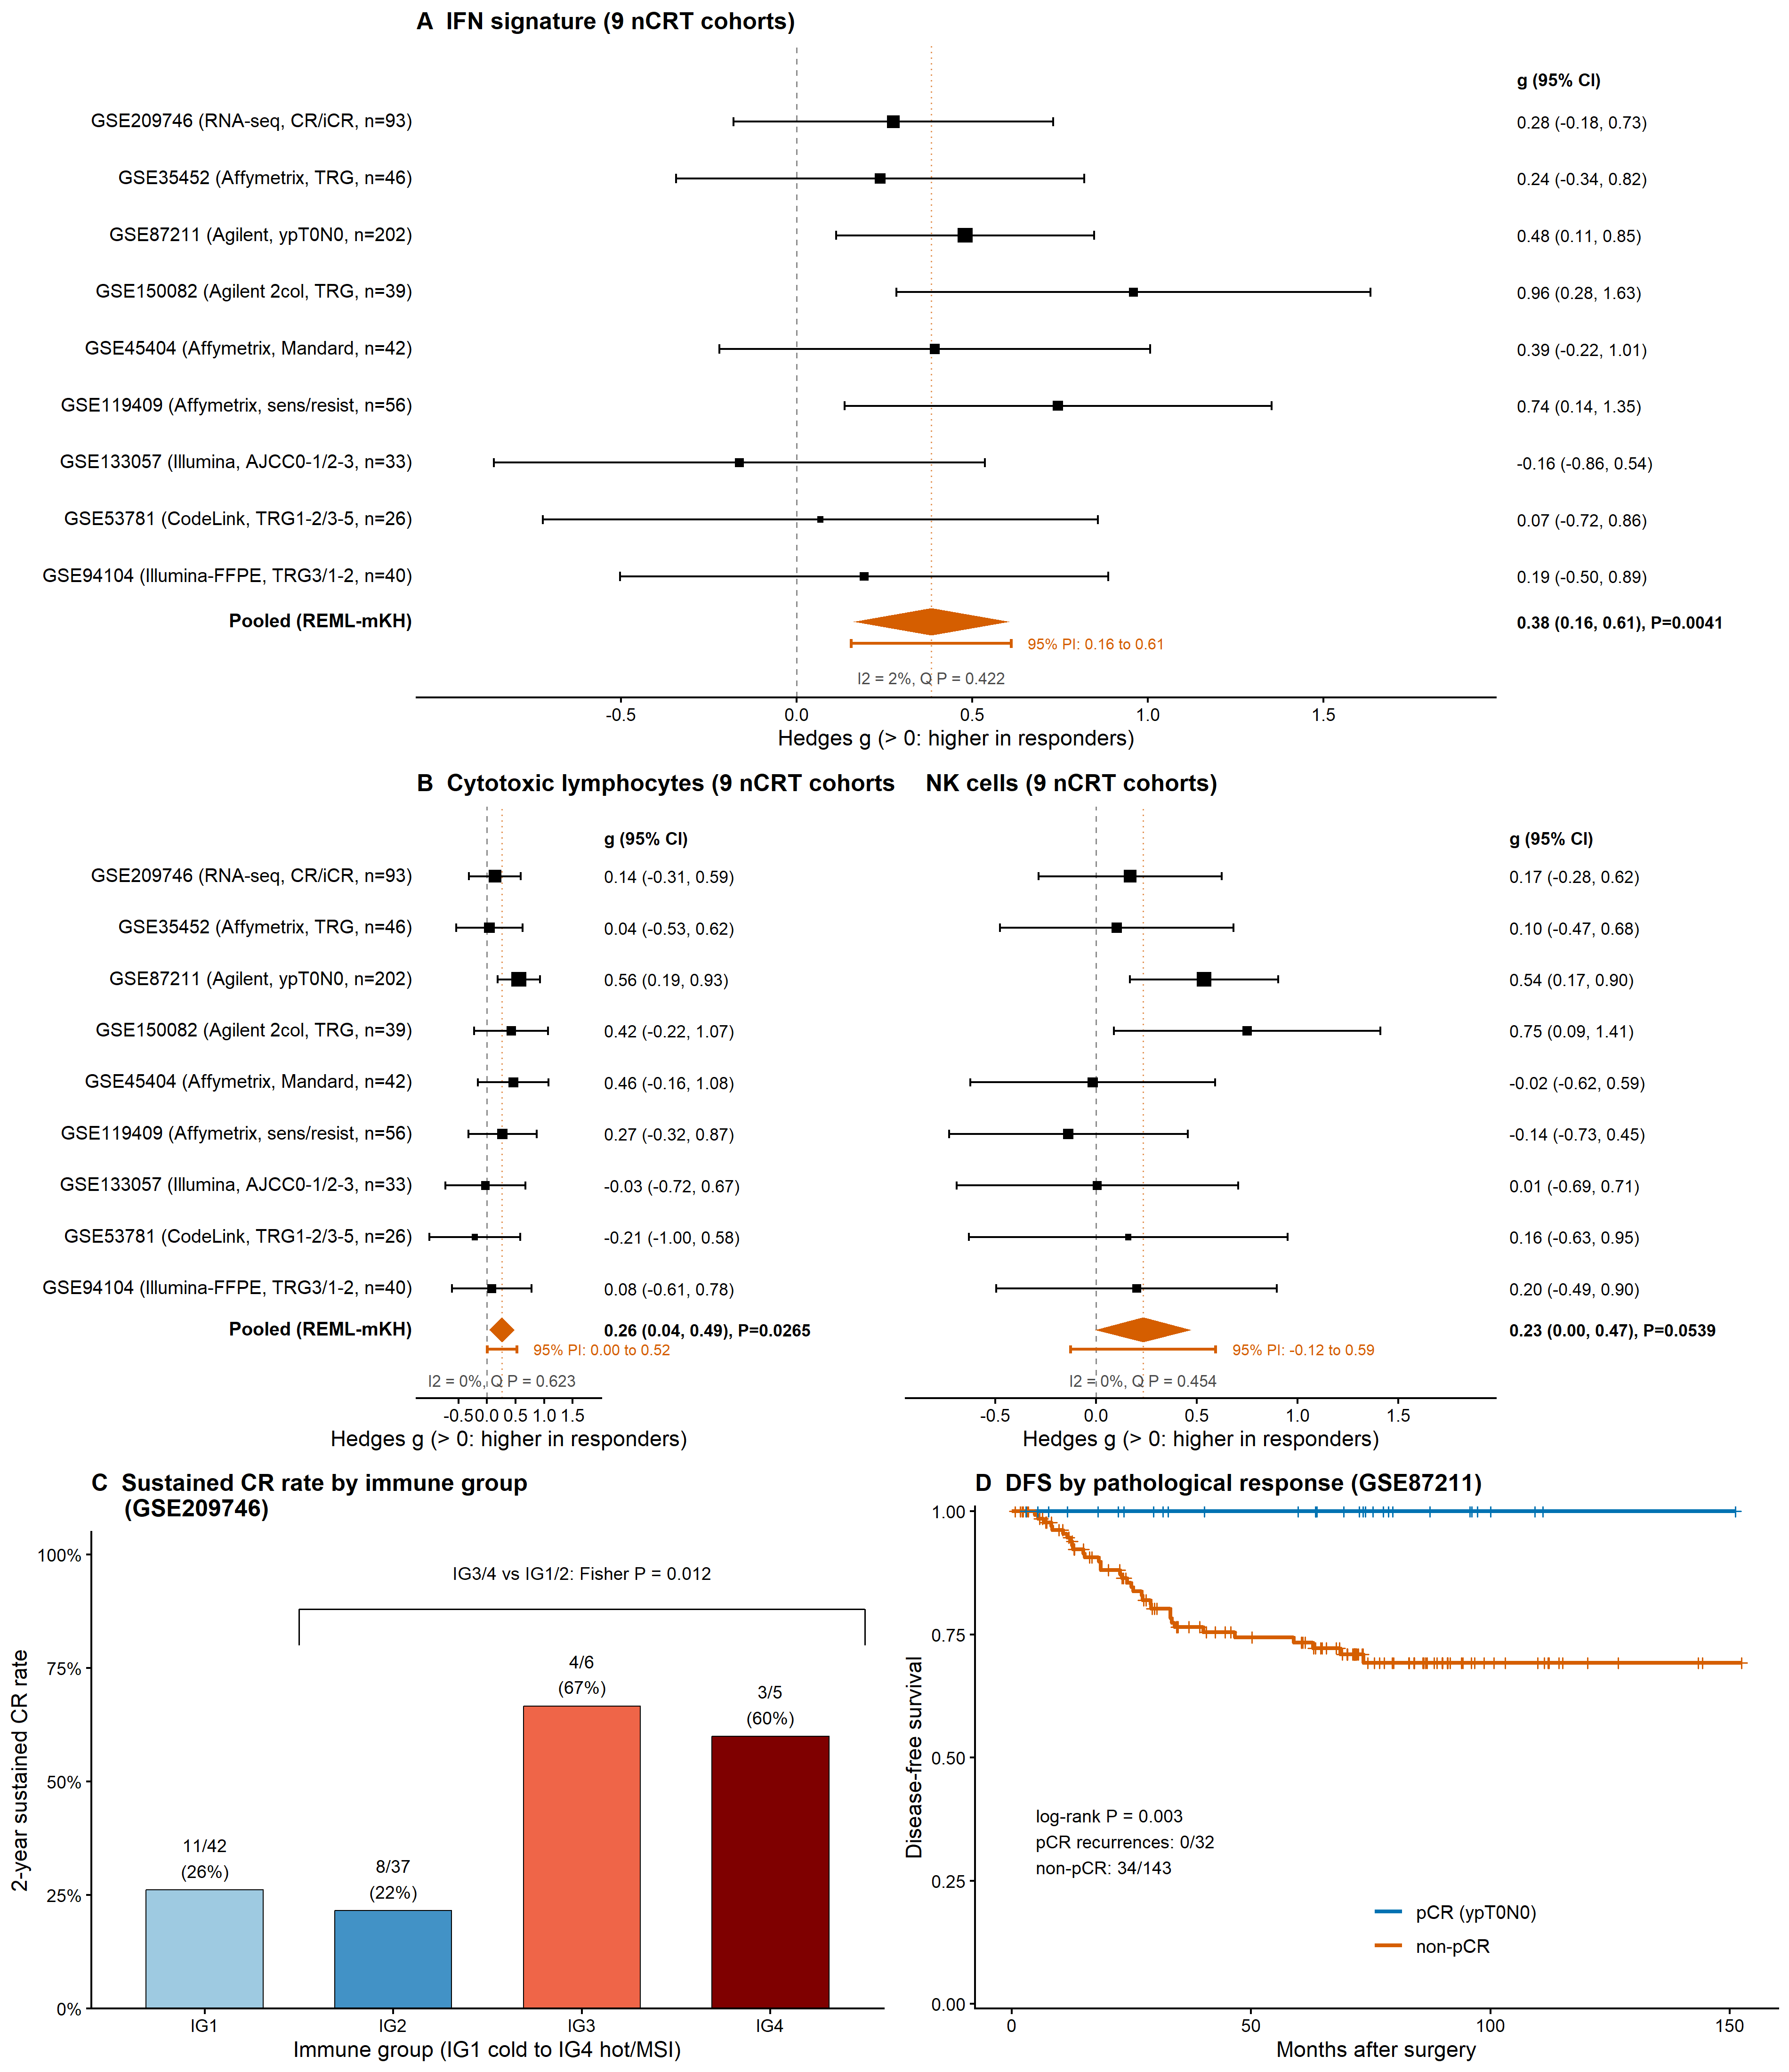
\includegraphics[width=\textwidth]{Fig1_main.png}
\caption{Cross-cohort evidence for an interferon and cytotoxic-immune theme of nCRT response. Throughout, positive Hedges $g$ indicates higher scores in responders.
\textbf{(A)} Forest plot of the pretreatment IFN score across nine nCRT cohorts. The diamond shows the REML estimate with its modified Hartung--Knapp confidence interval ($g=0.38$, 95\% CI 0.16--0.61; $P=0.0041$; $I^2=1\%$). The orange bar shows the 95\% prediction interval, which nearly coincides with the confidence interval because $\tau^2\approx0$.
\textbf{(B)} Forest plots for cytotoxic-lymphocyte and NK-cell marker-set scores (cytotoxic $g=0.26$, $P=0.026$; NK $g=0.23$, $P=0.054$).
\textbf{(C)} Complete-response rates by reconstructed immune group in GSE209746 (IG3/4 versus IG1/2; Fisher $P=0.012$).
\textbf{(D)} Disease-free survival by pathological response in GSE87211. Patients with pCR had no observed recurrences (0/32), compared with 34 events among 143 non-pCR patients over a median 71.2-month follow-up (log-rank $P=0.003$).}
\label{fig:main}
\end{figure}

% ---------------- Figure legends (S) ----------------
\section*{Supplementary figure legends}

\noindent\textbf{Figure S0.} PRISMA-style flow of systematic cohort identification (41 assessed, 31 excluded, nine nCRT cohorts in the primary synthesis plus one radiotherapy sensitivity cohort). GSE213331 was excluded after audit because its response-labelled samples are post-treatment resections.

\vspace{0.3em}
\noindent\textbf{Figure S1.} Hallmark pathway consistency (camera); signed $-\log_{10}(P)$ values show directions and strengths across four initial cohorts, with positive values indicating upregulation in responders.

\vspace{0.3em}
\noindent\textbf{Figure S2.} Meta-analysis diagnostics: leave-one-cohort-out influence, funnel plots with Egger tests, and Baujat influence plots (heterogeneity contribution vs influence on the pooled estimate).

\vspace{0.3em}
\noindent\textbf{Figure S3.} Forest plots for the within-cohort top-tertile score sensitivity analysis, pooled OR.

\vspace{0.3em}
\noindent\textbf{Figure S4.} (A) ROC curves of the IFN score in three cohorts (GSE209746, GSE35452, GSE87211); the GSE150082 AUC (0.764) was computed in the same pipeline and is reported in the text without a plotted curve. (B) Fixed-coefficient IFN+\textit{IGF2}+\textit{L1CAM} transfer model, trained in GSE209746 and applied without refitting to GSE35452 and GSE87211.

\vspace{0.3em}
\noindent\textbf{Figure S5.} Fifteen-gene signature gene-level REML-mKH meta-analysis; no gene survived BH correction.

\vspace{0.3em}
\noindent\textbf{Figure S6.} (A) Natural-spline fit of DFS hazard versus IFN score in GSE87211 (non-linearity $P=0.44$). (B) TCGA-READ overall survival Kaplan--Meier context by median IFN score.

\vspace{0.3em}
\noindent\textbf{Figure S7.} Robustness of the IFN association across nine nCRT cohorts. Pooled effects are shown for the primary Hallmark score, three alternative IFN signatures and five core genes. Positive $g$ indicates higher values in responders.

\vspace{0.6em}
\noindent\textbf{Supplementary tables.} S1, response-definition harmonization per cohort; S2, platform and preprocessing harmonization chain; S3, 15-gene per-cohort and pooled effects; S4, leave-one-cohort-out results; S5, top-tertile dichotomization tables; S6, confounder-adjustment models (stroma, MSI, WES purity/TMB/CNA, KRAS); S7, GSE87211 and TCGA-READ Cox models; S8, IFN-signature robustness across alternative signatures and core genes; S9, implementation sensitivity (mean-$z$ scoring and official MCPcounter package); S10, response-definition subgroup pooling and GSE87211 regimen sensitivity. Supplementary Methods: full systematic-search record.

% ---------------- References ----------------
\begin{thebibliography}{31}
\small
\setlength{\itemsep}{1pt}

\bibitem{Sauer} Sauer R, Becker H, Hohenberger W, et al. Preoperative versus postoperative chemoradiotherapy for rectal cancer. N Engl J Med 2004;351:1731--1740. PMID 15496622.

\bibitem{GarciaAguilar} Garcia-Aguilar J, Patil S, Gollub MJ, et al. Organ preservation in patients with rectal adenocarcinoma treated with total neoadjuvant therapy. J Clin Oncol 2022;40:2546--2556. PMID 35483010.

\bibitem{Akiyoshi} Akiyoshi T, Wang Z, Kaneyasu T, et al. Transcriptomic analyses of pretreatment tumor biopsy samples, response to neoadjuvant chemoradiotherapy, and survival in patients with advanced rectal cancer. JAMA Netw Open 2023;6:e2252140. PMID 36662520.

\bibitem{Chatila} Chatila WK, Kim JK, Walch H, et al. Genomic and transcriptomic determinants of response to neoadjuvant therapy in rectal cancer. Nat Med 2022;28:1646--1655. PMID 35970919.

\bibitem{Alderdice} Alderdice M, Dunne PD, Cole AJ, et al. Natural killer-like signature observed post therapy in locally advanced rectal cancer is a determinant of pathological response and improved survival. Mod Pathol 2017;30:1287--1298. PMID 28621318.

\bibitem{Isella} Isella C, Terrasi A, Bellomo SE, et al. Stromal contribution to the colorectal cancer transcriptome. Nat Genet 2015;47:312--319. PMID 25706627.

\bibitem{Hu} Hu Y, Gaedcke J, Emons G, et al. Colorectal cancer susceptibility loci as predictive markers of rectal cancer prognosis after surgery. Genes Chromosomes Cancer 2018;57:140--149. PMID 29119627.

\bibitem{Watanabe} Watanabe T, Kobunai T, Akiyoshi T, et al. Prediction of response to preoperative chemoradiotherapy in rectal cancer by using reverse transcriptase polymerase chain reaction analysis of four genes. Dis Colon Rectum 2014;57:23--31. PMID 24316942.

\bibitem{Sendoya} Sendoya JM, Iseas S, Coraglio M, et al. Pre-existing tumoral B cell infiltration and impaired genome maintenance correlate with response to chemoradiotherapy in locally advanced rectal cancer. Cancers (Basel) 2020;12:2208. PMID 32784964.

\bibitem{Agostini} Agostini M, Zangrando A, Pastrello C, et al. A functional biological network centered on XRCC3: a new possible marker of chemoradiotherapy resistance in rectal cancer patients. Cancer Biol Ther 2015;16:1160--1171. PMID 26023803.

\bibitem{Palma} Palma P, Cano C, Conde-Mui\~no R, et al. Expression profiling of rectal tumors defines response to neoadjuvant treatment related genes. PLoS One 2014;9:e112189. PMID 25380052.

\bibitem{Ji} Ji D, Song C, Li Y, et al. Combination of radiotherapy and suppression of Tregs enhances abscopal antitumor effect and inhibits metastasis in rectal cancer. J Immunother Cancer 2020;8:e000826. PMID 33106387.

\bibitem{Ferrandon} Ferrandon S, DeVecchio J, Duraes L, et al. CoA synthase (COASY) mediates radiation resistance via PI3K signaling in rectal cancer. Cancer Res 2020;80:334--346. PMID 31704889.

\bibitem{He} He L, Jin M, Jian D, et al. Identification of four immune subtypes in locally advanced rectal cancer treated with neoadjuvant chemotherapy for predicting the efficacy of subsequent immune checkpoint blockade. Front Immunol 2022;13:955187. PMID 36238279.

\bibitem{Love} Love MI, Huber W, Anders S. Moderated estimation of fold change and dispersion for RNA-seq data with DESeq2. Genome Biol 2014;15:550. PMID 25516281.

\bibitem{Hanzelmann} H\"anzelmann S, Castelo R, Guinney J. GSVA: gene set variation analysis for microarray and RNA-seq data. BMC Bioinformatics 2013;14:7. PMID 23323831.

\bibitem{Liberzon} Liberzon A, Birger C, Thorvaldsd\'ottir H, et al. The Molecular Signatures Database (MSigDB) hallmark gene set collection. Cell Syst 2015;1:417--425. PMID 26771021.

\bibitem{Becht} Becht E, Giraldo NA, Lacroix L, et al. Estimating the population abundance of tissue-infiltrating immune and stromal cell populations using gene expression. Genome Biol 2016;17:218. PMID 27765066.

\bibitem{Bindea} Bindea G, Mlecnik B, Tosolini M, et al. Spatiotemporal dynamics of intratumoral immune cells reveal the immune landscape in human cancer. Immunity 2013;39:782--795. PMID 24138885.

\bibitem{Wu} Wu D, Smyth GK. Camera: a competitive gene set test accounting for inter-gene correlation. Nucleic Acids Res 2012;40:e133. PMID 22638577.

\bibitem{Ritchie} Ritchie ME, Phipson B, Wu D, et al. limma powers differential expression analyses for RNA-sequencing and microarray studies. Nucleic Acids Res 2015;43:e47. PMID 25605792.

\bibitem{Ayers} Ayers M, Lunceford J, Nebozhyn M, et al. IFN-$\gamma$-related mRNA profile predicts clinical response to PD-1 blockade. J Clin Invest 2017;127:2930--2940. PMID 28650338.

\bibitem{IntHout} IntHout J, Ioannidis JPA, Rovers MM, Goeman JJ. Plea for routinely presenting prediction intervals in meta-analysis. BMJ Open 2016;6:e010247. PMID 27406637.

\bibitem{Robin} Robin X, Turck N, Hainard A, et al. pROC: an open-source package for R and S+ to analyze and compare ROC curves. BMC Bioinformatics 2011;12:77. PMID 21414208.

\bibitem{Liu} Liu J, Lichtenberg T, Hoadley KA, et al. An integrated TCGA pan-cancer clinical data resource to drive high-quality survival outcome analytics. Cell 2018;173:400--416. PMID 29625055.

\bibitem{Corro} Corr\`o C, Carvalho J, Rapti M, et al. Integrative analysis of transcriptomic data reveals a predictive gene signature for chemoradiotherapy response in rectal cancer. iScience 2026;29:114455. PMID 41550766.

\bibitem{Wang} Wang Q, Tian N, Guo H, et al. Tumor stroma-immune interactions shape the immunosuppressive microenvironment and predict response to neoadjuvant chemoradiotherapy plus immunotherapy in rectal cancer. J Immunother Cancer 2026;14:e015376. PMID 42547264.

\bibitem{Rajamanickam} Rajamanickam V, Simons ND, Rosales W, et al. CMS subtypes correlate with complete response in trial of neoadjuvant galunisertib plus chemoradiation in rectal cancer. Transl Oncol 2026;66:102690. PMID 41653703.

\bibitem{Cercek} Cercek A, Lumish M, Sinopoli J, et al. PD-1 blockade in mismatch repair-deficient, locally advanced rectal cancer. N Engl J Med 2022;386:2363--2376. PMID 35660797.

\bibitem{Xue} Xue Z, Yang S, Luo Y, et al. An immuno-score signature of tumor immune microenvironment predicts clinical outcomes in locally advanced rectal cancer. Front Oncol 2022;12:993726. PMID 36248969. (GSE39582 usage unverifiable; see Discussion~4.5.)

\bibitem{Marisa} Marisa L, de Reyni\`es A, Duval A, et al. Gene expression classification of colon cancer into molecular subtypes: characterization, validation, and prognostic value. PLoS Med 2013;10:e1001453. PMID 23700391.

\end{thebibliography}

\end{document}
